\chapter{Introduction and Background}

\section{Motivation}

In the direct numerical simulation (DNS) of fluid systems,
the aim is to resolve the smallest features of the flow
without resorting to any modeling of the turbulence.
This involves the use of
extremely fine computational grids to
discretize the flow domain,
and some numerical method for solving the
flow equations on this grid.
Among the most popular numerical approaches for
solving the flow equations
is the \emph{finite difference method}.
The finite difference method approximates the
spatial and temporal derivatives appearing in the
partial differential equations that describe the flow
using finite difference schemes.
\emph{Compact finite difference schemes} are a class
of finite difference schemes that have found widespread
adoption in DNS codes
for their high order of accuracy and small stencil widths.
The evaluation of compact finite differences
requires the repeated solution of \emph{banded} linear systems,
making them fairly complex and expensive computationally.

When solving for flows numerically,
at each of the grid points in the computational domain,
various data about the flow must be stored---for
example, the geometric coordinates (x, y and z),
pressure, temperature and velocities at that point.
For even small problem sizes,
the amount of memory required to store this data
can quickly exceed the capacity of modern workstations/PCs.
Thus, a \emph{distributed memory} parallel system
is generally required for performing DNS.
Here, the traditional approach has been
to distribute parallel tasks among individual CPU cores,
or groups of CPU cores
that share common memory spaces.
In the latter case,
each group of cores constitutes a \emph{shared memory} system,
and the overall system is referred to as a \emph{hybrid system}.

The workhorse for computation in the above described
parallel systems is the CPU core,
however, more recently,
Graphics Processing Units (GPUs)
are being used for performing intensive calculations.
GPUs, while themselves being highly parallel processors,
can also function as accelerators in distributed memory systems
(GPU clusters).
However,
applications that exploit such systems
need careful redesign of algorithms---and
sometimes, substantial changes to code---to
see significant performance improvements.
This is because the CPU and GPU have very different architectures,
and any na\"{\i}ve ``parallelization'' of algorithms
designed for the CPU
is likely not take full advantage of the GPU's
memory hierarchy and compute ability.

The objective of this work is to develop an
approach for evaluating
compact finite differences---and
other numerical schemes leading to tridiagonal systems---on
multiple GPUs in a distributed system.
This is of interest because
the evaluation of spatial derivatives using
compact finite difference schemes is one of the most
expensive tasks in DNS.
But perhaps more significantly,
it encompasses several computational patterns
such as pointwise updates, stencil evaluations,
and solutions of distributed tridiagonal systems.
Efficient implementation of these computational patterns
on GPUs is of interest in other areas of CFD,
and scientific computation in general.

\section{Compact finite differences}

Numerical evaluation of derivatives is a central component
in scientific computing.
The simplest and most widely-used approach for numerical differentiation
is the \emph{finite difference} approximation,
wherein the numerical approximation of the derivative
is expressed as a \emph{difference equation}.
A key application of the finite difference approximation
is in \emph{finite difference methods},
a family of numerical methods for solving differential equations
in which the derivatives are approximated using
finite difference approximations.
%
For example, we may consider a uniformly sampled
function $f(x)$,
sampled at points $x_1, x_2, x_3, \hdots x_n$.
At each sample point $i$, we may approximate the derivative as
a combination of the function values at
$i$, and its neighbouring points:

\begin{enumerate}
    \item When the derivative at $i$ is expressed
        as some combination of the function values
        at $i$, $i+1$, $i+2$, $\hdots$,
        we refer to the approximation as a
        \emph{forward} difference.
        
    \item When the derivative is expressed as
        some combination of the function values
        at $i$, $i-1$, $i-2$, $\hdots$,
        we refer to the approximation as a
        \emph{backward} difference.

    \item When the derivative is expressed as
        some combination of the function values
        on \emph{both} sides of $i$, i.e,
        at $\hdots$, $i-2$, $i-1$, $i$, $i-1$, $i-2$, $\hdots$,
        we refer to the approximation as a
        \emph{central} difference.
\end{enumerate}
%
The approximation of higher order derivatives generally requires
inclusion of a larger number of points in the
finite difference approximation
(referred to as the finite difference \emph{stencil}).
For a given order of derivative,
finite difference approximation of arbitrary stencil widths
may be derived,
with larger stencils associated with higher accuracy \cite{fornberg1988generation}.
In the evaluation of spatial derivatives,
the above schemes are referred to as \emph{explicit}
schemes, as the derivative at each point
can be expressed as some explicit combination of function values.

\subsection{General form of compact finite difference schemes}
\label{subsec:gen-form-compact}

Compact schemes express the derivative at a point $i$
in terms of
function values \emph{and derivatives}
at neighbouring points,
i.e., the derivative is expressed \emph{implicitly}.
For example,
if $f_i$ represents the value of
a uniformly sampled function evaluated at the $i$th sample point,
the first derivative $f^{\prime}_i$ can be approximated from
a relation of the form:
%
\begin{equation}
\begin{split}
    f_i^{\prime} + \
    \alpha(f^{\prime}_{i-1} + f^{\prime}_{i+1}) + \
    \beta(f^{\prime}_{i-2} + f^{\prime}_{i+2}) + \
    \hdots
    = 
    a\frac{f_{i+1} - f_{i-1}}{h} + \
    b\frac{f_{i+2} - f_{i-2}}{h} + \\
    c\frac{f_{i+3} - f_{i-3}}{h} + \
    \hdots
\end{split}
\label{eqn:general-compact}
\end{equation}
%
where $\alpha$, $\beta$, $a$, $b$, $c$, etc.,
are parameters that must satisfy certain constraints \cite{kennedy1994several,lele1992compact},
and $h$ is the space between two grid points.
We note that for equations of the form in Eq. (\ref{eqn:general-compact}),
the derivative at any points $i$ cannot be computed explicitly.
Instead, we must write similar equations for \emph{all} points $i$
in the range.
This results in a system of linear equations
with unknowns \{$f^{\prime}_1$, $f^{\prime}_2$, $\hdots$, $f^{\prime}_n$\},
which may be represented by the matrix system $A\bm{x}=\bm{d}$,
where $\bm{x}$ is the vector
\{$f^{\prime}_1$, $f^{\prime}_2$, $\hdots$, $f^{\prime}_n$\},
$\bm{d}$ is a vector of right hand sides [Eq. (\ref{eqn:general-compact})],
and $A$ is, in general, a \emph{banded} matrix.

\subsection{Wavenumber analysis of finite difference methods}
\label{subsec:wavenumber-analysis}

For DNS applications, the relevant measure of accuracy of a
finite difference scheme is obtained from the so-called
\emph{modified wavenumber} approach.
Here, we test the scheme's ability to
accurately estimate the derivative of sinusoidal functions
with increasing wavenumbers (frequencies),
given a specified grid size. 
We expect that the approximation of the derivative
becomes more difficult with increasing wavenumbers,
as the function value varies more rapidly.
The wavenumber of the approximate derivative
as given by the finite difference scheme is compared with
the wavenumber of the exact derivative.
The result for different schemes is shown
in Fig. \ref{fig:modified-wavenumbers}.

\begin{figure}
\begin{center}
\includegraphics[height=250pt]{fig/modified-wavenumbers.eps}
\end{center}
\caption{Modified wavenumbers for different finite difference schemes.
    $k^\prime$ is the wavenumber of the approximated derivative,
    while $k$ is wavenumber of the exact derivative.
    $h$ represents the spacing between two grid points.
    The compact schemes better estimate the derivative
    for higher wavenumbers.}
\label{fig:modified-wavenumbers}
\end{figure}

The ability of a finite difference scheme
to accommodate large wavenumbers
is extremely relevant in
computational fluid dynamics applications
\cite{KravchenkoEffNumErr}.
In DNS, the scheme
\emph{must} capture the
rapidly varying characteristics of the flow
associated with the turbulence.
For this purpose,
higher order explicit schemes
may be considered.
While they are straightforward to compute,
they are associated with large stencil widths.
In most applications,
large stencil widths are undesirable.
This is because
the arithmetic intensity increases with stencil size, i.e.,
a larger number of computations must be performed per grid point.
Further,
the amount of boundary information that must be exchanged
between parallel processes increases,
which can seriously affect overall performance.

From Fig. \ref{fig:modified-wavenumbers},
it is clear that the compact schemes are better
able to compute derivatives for larger wavenumbers
for a given stencil width.
This makes them the superior choice for DNS,
in which the flow quantities
exhibit spatial variation associated with high wavenumbers.

\subsection{Boundary conditions}

One of the advantages of the compact finite difference approach
is that it accommodates \emph{non-periodic} boundary conditions.
This is in contrast to other methods used in DNS,
such as \emph{spectral} methods.
We note that the Eq. (\ref{eqn:general-compact})
cannot be applied near the boundary points.
At the boundaries,
\emph{non-centered} or \emph{one-sided}
finite difference approximations are required.
Some considerations are made in choosing
these approximations:
firstly, the bandwidth of the resulting banded matrix
must be preserved.
Secondly,
the width of the boundary stencils
must be lower than the interior stencils,
as higher order boundary stencils are unstable
\cite{kennedy1994several}.
In general, boundary equations for the first derivative
are of the following form \cite{lele1992compact}:

\begin{equation}
    f_1^{\prime} + \alpha^{\prime}f_2^{\prime} = \
        \frac{1}{h}(a^{\prime}f_1 + b^{\prime}f_2 + c^{\prime}f_3 + d^{\prime}f_4)
\label{eqn:boundary-compact}
\end{equation}

\subsection{Tridiagonal compact schemes}
\label{sec:tridiagonal-compact-schemes}

As mentioned in Sec. \ref{subsec:gen-form-compact},
compact finite difference schemes lead to
\emph{banded} linear systems.
The simplest classes of banded matrix include
diagonal, tridiagonal and pentadiagonal matrices.
When $\alpha$ = $\beta$ = $\hdots$ = 0,
$A$ is a $\emph{diagonal}$ matrix.
In this case, the
scheme is \emph{explicit}
and the derivatives are straightforward to evaluate:
this simply involves the
application of the right-hand side stencil at each point.
When $\alpha \neq 0, \beta = \hdots$ = 0,
$A$ is tridiagonal.
The evaluation of the derivatives requires
the solution of the resulting tridiagonal system.
When $\alpha \neq 0$ and $\beta \neq  0$,
pentadiagonal systems arise.
These can be more expensive and difficult to evaluate
than tridiagonal systems
using a direct method.

This work will focus on
compact finite difference schemes that lead
to tridiagonal systems.
An example of such a scheme is obtained
by substituting 
$\beta = 0$, $\alpha = \frac{1}{4}$ and $a = \frac{3}{4}$
in Eq. (\ref{eqn:general-compact})
(all other coefficients are set to zero).
This leads to a fourth-order accurate
tridiagonal compact finite difference scheme,
known also as the Pad\'{e} scheme.
At the boundaries,
the following \emph{third-order} accurate
approximations are used:

\begin{align}
    f^{\prime}_1 + 2f^{\prime}_2 &= \frac{-5f_1 + 4f_2 + f_3}{dx} \\
    f^{\prime}_{n} + 2f^{\prime}_{n-1}
    &=
    \frac{5f_{n} - 4f_{n-2} -  f_{n-1}}{dx}
\end{align}
%
The resulting tridiagonal system is then:

\begin{equation}
 \label{eqn:compact-tridiagonal-system}
 \begin{bmatrix}
     1&2\\
     1/4&1&1/4\\
     &1/4&1&1/4\\
     &&1/4&1&1/4\\
     &&&1/4&1&1/4\\
     &&&&&\ddots\\
     &&&&&&\ddots\\
     &&&&&&&\ddots\\
     &&&&&&&2&1
  \end{bmatrix}
  \begin{bmatrix}
      f^{\prime}_1 \\

      f^{\prime}_2 \\
      f^{\prime}_3 \\
      \vdots \\
      \vdots \\
      \vdots \\
      \vdots \\
      f^{\prime}_{n-1} \\
      f^{\prime}_n
   \end{bmatrix}
 =
 \begin{bmatrix}
     \frac{-5f_1 + 4f_2 + f_3}{2dx}\\
     \frac{3(f_{3} - f_{1})}{4dx}\\
     \frac{3(f_{4} - f_{2})}{4dx}\\
     \vdots\\
     \vdots\\
     \vdots\\
     \vdots\\
     \frac{3(f_{n} - f_{n-2})}{4dx}\\
     \frac{5f_{n} - 4f_{n-1} - f_{n-2}}{2dx}
  \end{bmatrix}
\end{equation}

Similar tridiagonal schemes are available
to evaluate higher order derivatives.
Compact schemes for
second, third and fourth derivatives
are derived in \cite{lele1992compact}.

\section{Graphics processing units}

The evolution of graphics processing units (GPUs)
has traditionally been guided by the requirements
of graphics applications such as video gaming.
In general, these graphics computations involve
manipulations and calculations with pixel data.
Because these calculations are largely independent,
the GPU hardware is specialized
to perform several of them \emph{in parallel}.
Therefore, the
GPU may be regarded as a highly multithreaded processor.
Initially,
programming GPUs for scientific computation tasks
was a cumbersome process,
as the programming interfaces were designed for graphics computations,
and attempts to use them for other purposes were essentially ``hacks''.
Moreover, there was little support for double precision arithmetic,
which is critical for many applications.
But with the introduction of the
NVIDIA Compute Unified Device Architecture (CUDA)
parallel computing platform
and programming model,
CUDA-enabled GPUs have come into the
mainstream in high-performance computing.
A history of the development of GPUs
for general purpose computation,
and of CUDA specifically is available
in \cite{HwuBook}.
We provide the essential and relevant details about CUDA here,
and refer to the
CUDA Programming Guide \cite{CUDAProgrammingGuide}
for a detailed outlook.

\subsection{The CUDA Programming model}

CUDA is the name for the parallel computing platform
developed by NVIDIA,
as well as the application programming interface
for programming their GPUs.
CUDA allows general-purpose applications to be
more easily programmed for the GPU.
Two essential features of the CUDA programming model
are \emph{kernels} and \emph{thread organization}.

\subsubsection{Kernels}

The CUDA application programming interface (API)
is available as an extension to
a programming languages (C, C++, Fortran, etc.),
allowing certain portions of code to execute on the GPU.
The rest of the code is executed as usual on the CPU.
In CUDA terminology,
the CPU is referred to as the \emph{host},
and the GPU is referred to as the \emph{device}.
The special pieces of code
that execute on the GPU are known as \emph{kernels}.
Kernels have similar syntax
as ``host code'',
but in general,
are more restricted in the
features of the underlying language they can use.
In C, for example, kernels are written as \emph{functions},
and are called by the host code
using (almost) the same conventions.
Thus, a C program that uses the GPU
looks and behaves very much like a normal C program,
but includes special calls to these kernels.
When the application is launched,
a CPU thread executes the host-code as usual,
but upon encountering a call to the kernel,
it passes program control over to the GPU.
After the kernel is finished executing,
control is passed back to the CPU,
and this process may repeat when another kernel call is encountered.
The CPU and GPU may also operate \emph{asynchronously},
i.e.,
control may be passed back to the CPU \emph{before} kernel completion,
in which case
explicit synchronization between the host and device may be necessary.
Apart from kernel calls, the host code can also call functions to
allocate and deallocate device memory,
query device information,
perform device synchronization, etc.

\subsubsection{Thread organization}

A kernel is executed in parallel by
several lightweight \emph{threads}.
Threads are organized into groups called
\emph{thread blocks}, or just \emph{blocks},
and the different blocks constitute a
\emph{grid} of blocks.
In many cases,
the GPU is used to process array data,
and each thread is mapped to a single array element.
In most applications,
the array is logically 1-, 2- or 3-dimensional.
Thus, for convenience, the grid and block sizes
can be 1-, 2- or 3-dimensional
(hence the terminology \emph{grid} and \emph{blocks}).
This kind of thread organization is optional,
and $n$-dimensional arrays can be processed
using just 1-dimensional grids and blocks.

\subsection{CUDA architecture and memory model}

\begin{figure}
\begin{center}
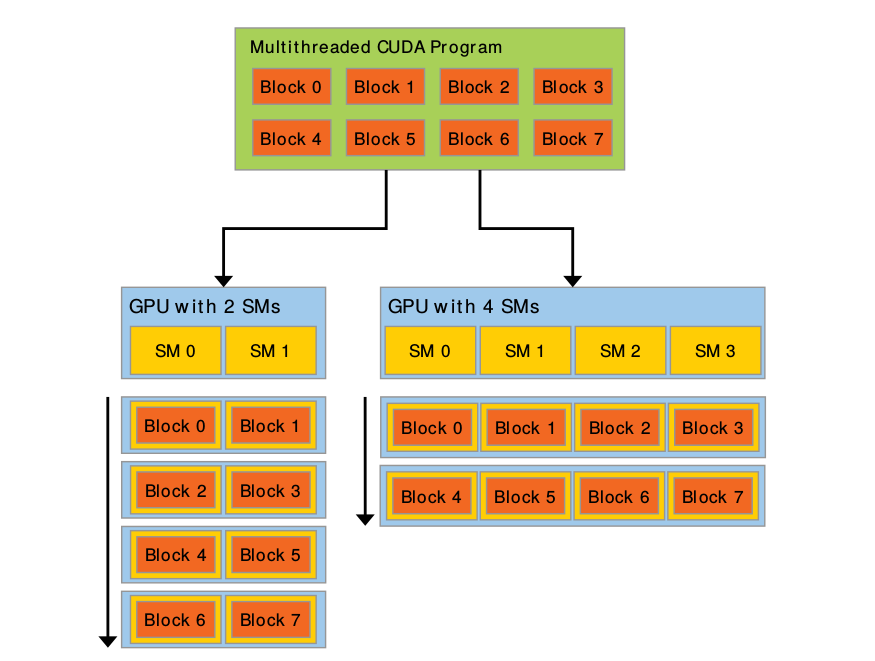
\includegraphics[height=250pt]{img/gpu-scaling.png}
\end{center}
\caption{Scheduling of blocks to streaming microprocessors---GPUs
    with more SMs are able to execute more blocks concurrently.
(\emph{CUDA Programming Guide \cite{CUDAProgrammingGuide}})}
\label{fig:gpu-scaling}
\end{figure}

From the hardware perspective,
an NVIDIA GPU may be viewed primarily as
a collection of so-called Streaming Microprocessors (SMs).
When a kernel is launched with specified
grid size (number of blocks)
and block size (threads per block),
each block is assigned to an SM.
Threads within a thread block can execute concurrently on the SM,
and an SM can execute several thread blocks concurrently.
It is imperative that blocks are able to run
independently, in series or in parallel.
This feature gives CUDA programs
their scalability (Fig. \ref{fig:gpu-scaling}).
The same program runs faster on a GPU with a larger number
of SMs, simply because more blocks may run concurrently.
The number of thread blocks that an
SM can execute concurrently
is limited by a number of factors,
and maximizing this number is often
key to obtaining good performance.
Another key consideration in the implementation
of algorithms on GPUs is the
available \emph{memory hierarchy}.
Threads executing a kernel can read and write
to several different memory spaces,
each with different capacity, latency and bandwidth.

\subsubsection{Global memory}

Data from the host is first read into the
device's \emph{global memory}.
Similarly, data from the device is read back into the host
from global memory.
This is done in the host-code
using special functions provided by the CUDA API 
(e.g., \texttt{cudaMemcpy}).
Data transfer between the host and the device is
extremely slow relative to data access within the device.
This data transfer rate is limited by the bandwidth
of the PCI-e bus between the host and device.
All threads executing a kernel can
read and write to locations in global memory,
and it is the largest memory space that is
writable by the device.
For example, the current NVIDIA Tesla K20 accelerator
has about 4 Gigabytes of usable global memory.
Thread access to global memory has a long latency
and it is especially inefficient when
successive threads in a block access memory locations
that are far apart.
Data in global memory remains persistent
throughout the execution of the program.

\subsubsection{Shared memory}
\label{subsubsec:shared-memory}

Threads within a block have access to a
common, fast \emph{shared memory}.
All threads within a block
can read and write to the block's shared memory,
but they may \emph{not} access
shared memory of another block.
Thread access to shared memory can be expected to be
much faster than access to global memory.
Data that may be repeatedly used in a kernel
are good candidates for placement in shared memory
The contents of shared memory are managed by the kernel code,
and for this reason,
shared memory is often viewed as explicitly managed cache.
Data in shared memory does \emph{not} persist after
kernel execution.

\begin{figure}
\begin{center}
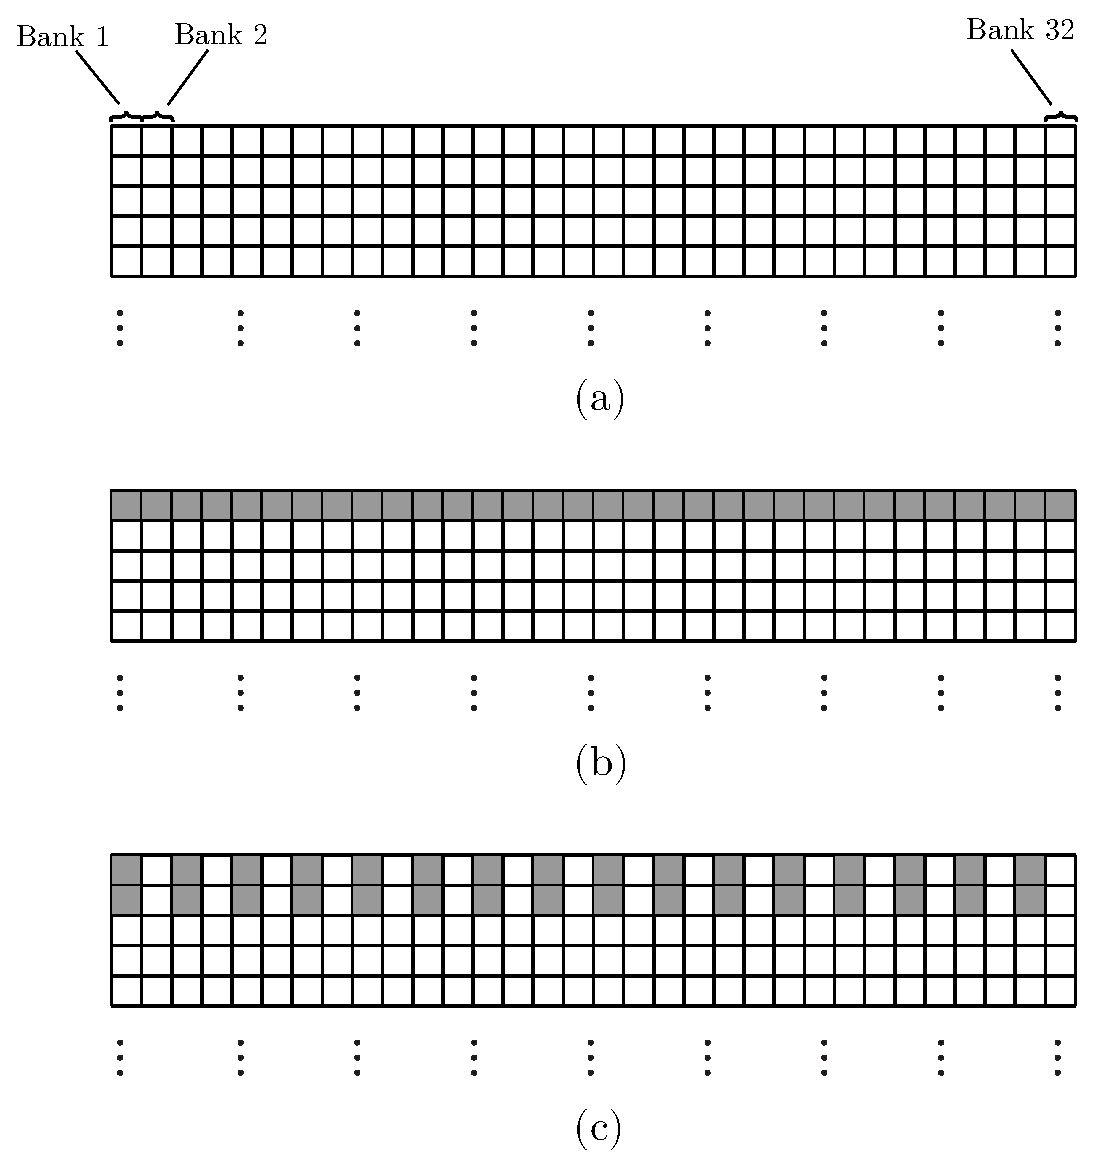
\includegraphics[height=300pt]{img/bank-conflicts.eps}
\end{center}
\caption{(a) Organization of shared memory as 4 byte words
    organized into 32 banks. Each cell (square) is a word.
    (b) Bank conflict free access by a warp. Each warp
    accesses a word from a different bank. (c) 2-way
    bank conflicts arising from successive threads accessing
alternating words.}
\label{fig:bank-conflicts}
\end{figure}

Shared memory is organized as a collection of  4 byte ``words''.
Each consecutive word in shared memory belongs
to a different bank - modern GPUs have 32 banks.
The GPU schedules
thread execution within a block
in groups of 32 (termed as thread \emph{warps}).
Ideally, these 32 threads
can access shared memory locations concurrently.
However, when two or more threads in a warp access
words from the same bank,
a \emph{bank conflict} is said to occur,
and the access is serialized.
Thus,
a warp of 32 threads reading
32 successive \texttt{float}s (4 bytes) in a shared memory array
is perfectly parallelized.
But a warp of 32 threads reading
32 alternating \texttt{float}s in a shared memory array
leads to bank conflicts (Fig. \ref{fig:bank-conflicts}).
Because the floats are placed in consecutive banks,
the 1st and 17th threads will access \texttt{float}s from the same bank,
as will the 2nd and 18th threads, and so on.
This specific kind of bank conflict is termed a
\emph{two-way} bank conflict -
threads access two words from the same bank.
It is observed that higher-order bank conflicts may occur,
if threads in a warp access
\texttt{float}s in strides of 4,
a \emph{four-way} bank conflict can occur.
In the worst case, successive threads may access
\texttt{float}s in strides of 32,
in which case all threads in the warp
request memory from the same bank:
a \emph{32-way} bank conflict.

\subsubsection{Registers and local memory}

Each thread also has private \emph{local memory},
and access to extremely fast registers.
Unlike CPUs, the GPU has a large number of registers---a
thread executing a kernel will
typically attempt to store
non-array variables defined in the kernel in registers.
Thread access to registers has the lowest latency
compared to all other memory spaces.
The number of registers available to each thread is limited,
and if exceeded,
data is instead stored in the thread's local memory.
Access to local memory is much slower than registers,
so this is typically avoided.

\subsubsection{Limiting shared memory and register usage}

While shared memory and registers can service memory requests
much faster than global memory,
their overuse can lead to performance degradation.
The amount of shared memory per SM
and the number of registers per SM is limited.
For the current NVIDIA Tesla K20 accelerator,
the amount of shared memory per SM is limited to 48 KiB,
and the number of registers per SM is limited to 65536.
These are also the limits
on the resources that can be allocated for each \emph{block}.
However,
allocating 48 KiB shared memory or using 65536 registers 
for each block is ill-advised,
as this effectively restricts the number of blocks that
each SM can run at any given time to 1.
If each block allocates 24 KiB of shared memory,
then an SM can run only 2 blocks concurrently.
Thus, the resources allocated per-block affects
the overall parallelism that can be exploited from the GPU.

\subsection{Considerations to be made while programming for GPUs}

As seen in the previous sections,
several factors must be considered while
designing and implementing algorithms for GPUs.
Failure to include these considerations can easily
lead to poor performance,
and no significant speedup may be noted over CPUs.
In fact, one may even note performance degradation.
We list the primary considerations here:

\begin{itemize}
    \item In any application, the data transfers between
        the host and device must be minimized.
        Ideally,
        data is read into the device from the host \emph{once}
        and from the device to the host \emph{once}.
    \item Thread access to global memory must be \emph{coalesced},
        i.e., successive threads must read successive locations
        in global memory.
    \item Shared memory access must be free of bank conflicts
        as much as possible---in general, this means avoiding
        strided shared memory access.
    \item The amount of shared memory and registers
        allocated for each block is kept minimum.
\end{itemize}

\section{Tridiagonal solvers for compact finite difference evaluation}

As mentioned in \ref{sec:tridiagonal-compact-schemes},
this work is concerned with
\emph{tridiagonal} compact finite differences
for their relative ease in evaluation.
The resulting tridiagonal system must be solved
repeatedly for all lines of grid points in the computational grid.
For a regular Cartesian grid (generally employed in DNS),
the coefficients of the tridiagonal systems
are the same for each grid line,
and only the right hand sides are different.
Thus, the compact finite difference evaluation
effectively requires the solution of a tridiagonal system
for several right hand sides.
In this section,
we describe the applicability of some algorithms
for solving this problem on the GPU.
We refer to \cite{chang2014guide} for
a more comprehensive list of algorithms,
along with details of their GPU implementation.

\subsection{Thomas algorithm}

\begin{equation} \label{eqn:general-tridiagonal-system}
\begin{pmatrix}
     b_1 & c_1  \\
     a_2 & b_2  &  c_2  \\
         & a_3  &  b_3 &  c_3  \\
         &      &  a_4 &  b_4 &  c_4  \\
         &      &      &      &  \ddots \\
         &      &      &      &     &  \ddots  \\
         &      &      &      &     &  a_n  &  b_n
\end{pmatrix}
\begin{bmatrix}
    x_1 \\
    x_2 \\
    x_3 \\
    x_4 \\
    \vdots \\
    \vdots \\
    x_n
 \end{bmatrix}
=
\begin{bmatrix}
   d_1 \\
   d_2 \\
   d_3 \\
   d_4 \\
   \vdots \\
   \vdots \\
   d_{n}
\end{bmatrix}
\end{equation}

Traditionally,
the Thomas algorithm is employed for solving
general linear systems of the form $A\bm{x} = \bm{d}$,
where $A$ is a tridiagonal matrix with diagonals
$\bm{a}$, $\bm{b}$ and $\bm{c}$
[Eq. (\ref{eqn:general-tridiagonal-system})].
The algorithm is derived
from the more general Gaussian (LU) algorithm
applied to tridiagonal matrices.
Implementations of this algorithm are relatively straightforward
and compact \cite{numericalrecipes}.
Only the non-zero diagonals of the tridiagonal matrix
are stored,
and the algorithm performs $2N$ steps
to solve the system.
It is also stable for diagonally dominant matrices.
The Thomas algorithm has an algorithmic complexity of $O(N)$,
and is the fastest serial solver for tridiagonal systems.
It is thus well suited to solution by a single CPU thread.
While the algorithm itself is sequential,
in a multithreaded environment,
the different CPU threads may be used to solve
the different independent tridiagonal systems simultaneously.

A similar parallelization strategy may be extended to GPUs,
where each GPU thread solves an independent tridiagonal system.
The coefficient right hand sides are assumed to be stored
contiguously as a single array in memory.
If each thread works entirely with global memory,
\emph{uncoalesced} memory access is observed.
This cost \emph{may} be amortized for a large enough
number of systems, as is the case
for 3-D problems \cite{sakharnykhADIconf}.
If shared memory is used,
then low parallelism is exhibited,
as the amount shared memory allocated by each thread
is relatively high ($4N$).
An approach that uses the parallel Thomas algorithm
effectively is described by Chang et al. \cite{chang2012scalable}.
Here, a \emph{parallel cyclic reduction} algorithm
is first used to reduce a
tridiagonal system into several smaller tridiagonal system,
and the parallel Thomas algorithm is then used to
solve the smaller systems in parallel.

\subsection{Cyclic reduction}

Two other popular algorithms for solving
tridiagonal systems are the
cyclic reduction (CR) and
the related parallel cyclic reduction (PCR)
algorithms.

\begin{figure}
\begin{center}
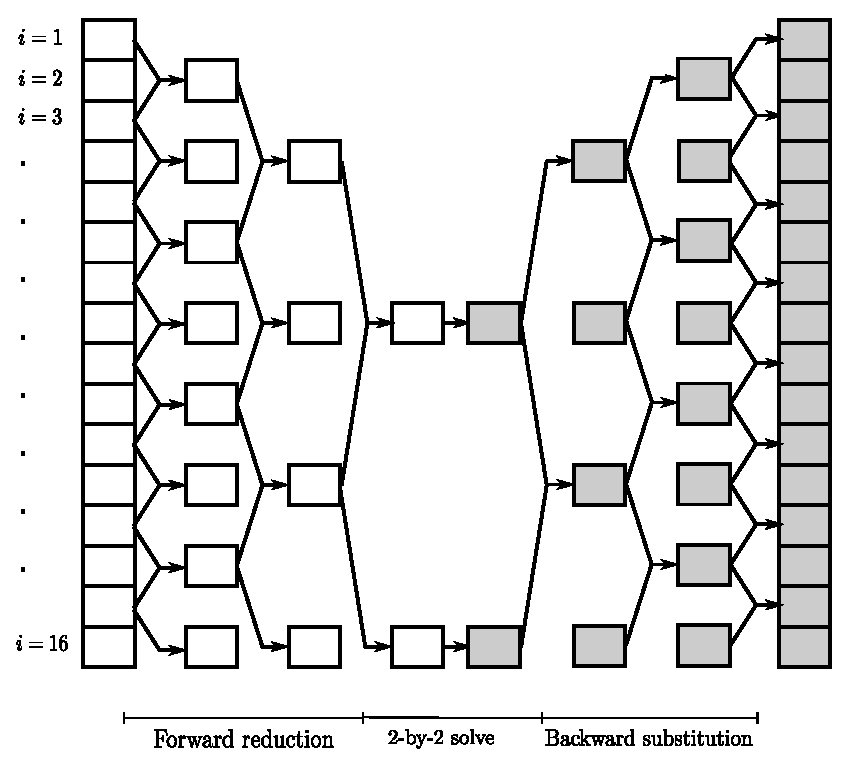
\includegraphics[height=250pt]{img/cyclic-reduction.eps}
\end{center}
\caption{Cyclic reduction.}
\label{fig:cyclic-reduction}
\end{figure}

The cyclic reduction algorithm consists of two phases:
\emph{forward reduction} and \emph{backward substitution}
(Fig. \ref{fig:cyclic-reduction}).
In the forward reduction phase,
every even-indexed equation $i$
is expressed as a
linear combination of equations $i$, $i-1$ and $i+1$,
yielding a new tridiagonal system of
$n/2$ equations in $n/2$ unknowns
[Eqs. (\ref{eqn:forward-reduction-1}) - (\ref{eqn:forward-reduction-4})].
The process is repeated until a system of
2 equations in 2 unknowns is left.

\begin{align} 
    a^{\prime}_i &= -a_{i-1}k_1 \
    \label{eqn:forward-reduction-1} \\
    b^{\prime}_i &= b_i - c_{i-1}k_1 - a_{i+1}k_2 \
    \label{eqn:forward-reduction-2} \\
    c^{\prime}_i &= -c_{i+1}k_2 \
    \label{eqn:forward-reduction-3} \\
    d^{\prime}_i &= d_i - d_{i-1}k_1  - d_{i+1}k_2 \
    \label{eqn:forward-reduction-4}
\end{align}
%
where,

\begin{align}
    k_1 &= \frac{a_i}{b_{i-1}} \label{eqn:k1-update} \\
    k_2 &= \frac{c_i}{b_{i+1}} \label{eqn:k2-update}
\end{align}

The 2-by-2 system of equations is solved trivially,
yielding $x_n$ and $x_{n/2}$.
In the backward substitution phase,
every odd-indexed unknown $x_i$ is solved for by
substituting the known values of $x_{i-1}$ and $x_{i+1}$
[Eq. (\ref{eqn:backward-substitution})].

\begin{equation} \label{eqn:backward-substitution}
x_i = \frac{d^{\prime}_i - a^{\prime}_ix_{i-1} - \
    c^{\prime}_ix_{i+1}}{b^{\prime}_i}
\end{equation}
%
For the last index $i=n$,
the forward reduction step is instead:
\begin{align} \label{eqn:forward-reduction-last}
    a^{\prime}_n &= -a_{n-1}k_1  \\
    b^{\prime}_n &= b_n - c_{n-1}k_1  \\
    d^{\prime}_n &= d_n - d_{n-1}k_1
\end{align}
%
And for $i=1$, the backward substitution step is instead:

\begin{equation} \label{eqn:backward-substitution-first}
x_1 = \frac{d^{\prime}_1 - c^{\prime}_1x_{2}}{b^{\prime}_1}
\end{equation}
%
In practice, the right-hand side vector can be safely
overwritten with the solution values
in backward substitution.

Thus, in the best case ($n$ parallel processors),
cyclic reduction requires 
$2log_2(n) - 1$ steps.
For even moderately large $n$,
this is significantly smaller than
the $2n$ steps required by the Thomas algorithm.
This makes cyclic reduction a good fit
for massively parallel architectures like GPUs.

\subsection{Parallel cyclic reduction}

The parallel cyclic reduction (PCR) algorithm
has only the forward reduction phase.
The first forward reduction step is applied to
the odd and even indexed equations seperately,
yielding two reduced systems
of size $n/2$.
Forward reduction applied to both of these
systems then yields \emph{four} reduced
systems of size $n/4$.
The process is repeated till
$n/2$ 2-by-2 systems are left,
all of which can be solved trivially.
The PCR algorithm requires half the number of steps
required by CR ($log_2(n)$),
but does significantly more computation per-step.
Further, unlike CR,
PCR can be implemented free of bank conflicts
\cite{Zhang2010FTS}.

\subsection{Cyclic reduction implementation on GPUs}
\label{subsec:cyclic-reduction-gpu-implementation}

The algorithm proposed in this work is based on cyclic reduction,
so it is pertinent to discuss the
implementation of cyclic reduction on GPUs,
the associated issues,
and the relevant literature.

\begin{figure}
\begin{center}
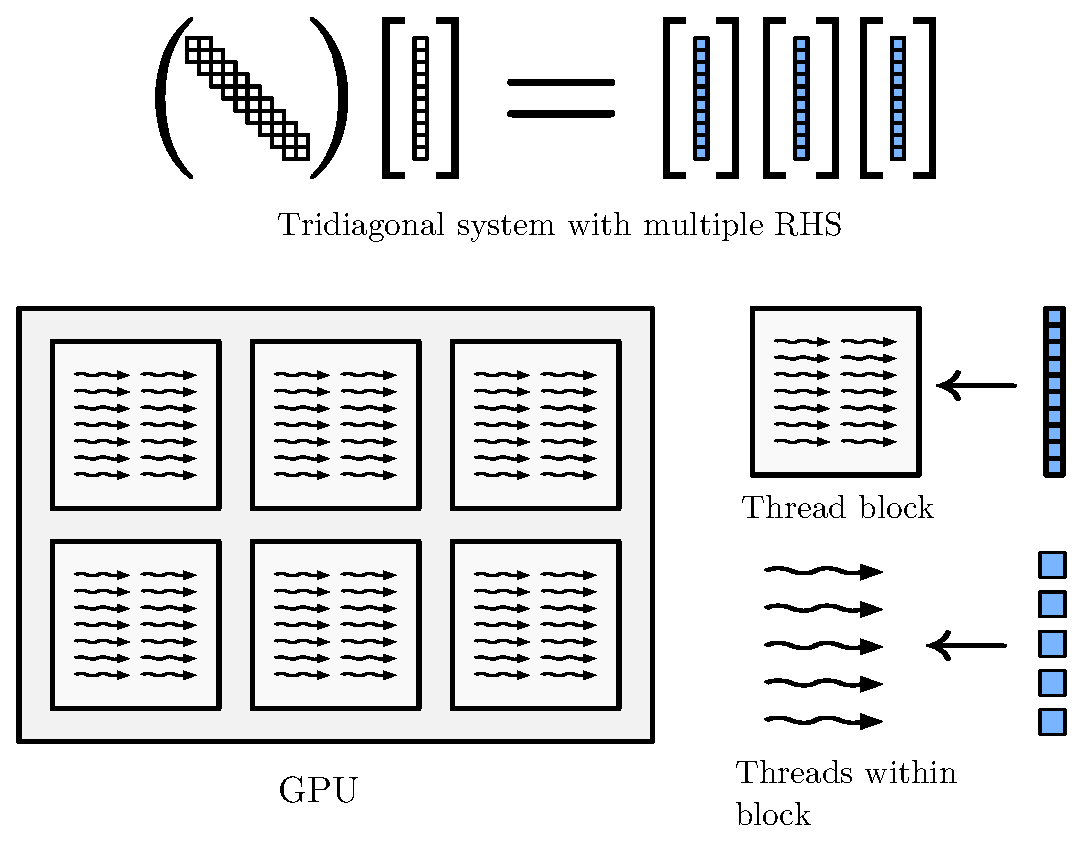
\includegraphics[height=200pt]{img/gpu-mapping.eps}
\end{center}
\caption{Mapping work to blocks and threads:
systems are mapped to blocks and
indices are mapped to individual threads.}
\label{fig:gpu-mapping}
\end{figure}
%
In the GPU implementation of cyclic reduction,
blocks are assigned to tridiagonal systems
(when solving multiple systems),
and threads within a block 
are assigned to equations, or \emph{indices}
(Fig. \ref{fig:gpu-mapping}).
In this way, several grid lines are solved concurrently
by the GPU.
During the forward reduction phase,
the threads assigned to each even index $i$
compute the coefficients
and right hand side for the reduced tridiagonal system
$a_i^\prime$, $b_i^\prime$ and $c_i^\prime$
and $d_i^\prime$.
In practice, the coefficients and right hand side
are updated \emph{in-place}.
Figure \ref{fig:forward-reduction-step} shows the updates
to the coefficient array $\bm{b}$
in the first forward reduction step,
a similar pattern is seen for the arrays
$\bm{a}$, $\bm{c}$ and $\bm{d}$.
In each step of forward reduction,
a thread accesses values from the
coefficient arrays and right hand side
in a \emph{strided} fashion.
At every subsequent step,
this stride is doubled, while the number of active threads is halved
\ref{fig:cyclic-reduction}.
In the backward substitution phase,
the strides are halved at each step,
while the number of active threads is doubled.

\begin{figure}
\begin{center}
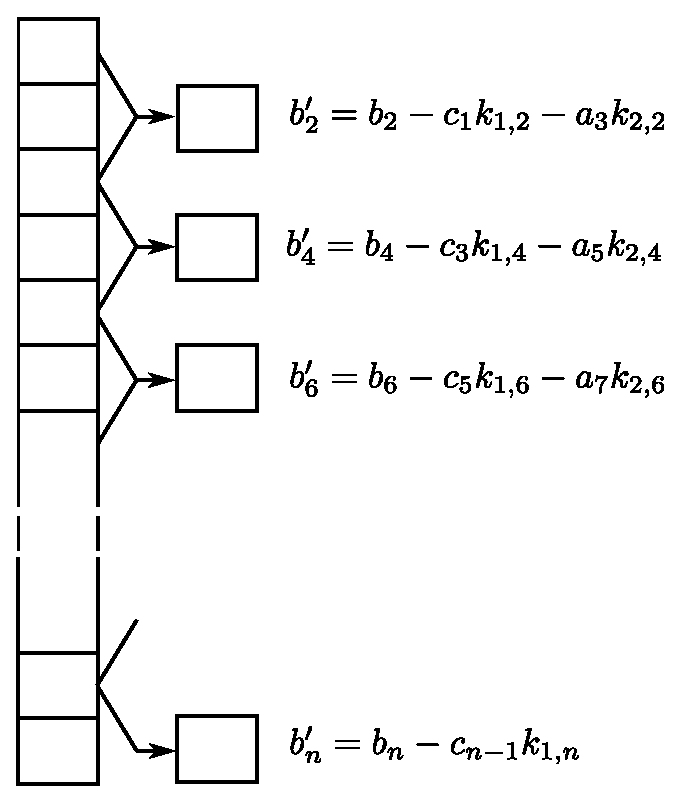
\includegraphics[height=200pt]{img/forward-reduction-step.eps}
\end{center}
\caption{Updating $\bm{b}$ in the first forward reduction step.}
\label{fig:forward-reduction-step}
\end{figure}

Several issues are encountered in the GPU implementation:

\begin{enumerate}
\item GPU utilization is low towards the end of forward reduction,
    and in the beginning of backward substitution.

\item Because coefficients and right hand sides
    are updated \emph{in-place},
    synchronization between the blocks is required at
    the end of each step.

\item If the threads work entirely with global memory,
    memory accesses are increasingly
    \emph{uncoalesced} in the forward reduction phase
    (and become increasingly coalesced in the
    backward substitution phase).

\item The use of shared memory prevents
    uncoalesced global memory access.
    Unfortunately,
    the power-of-two strides at each successive
    leads to bank conflicts,
    as described in Sec. \ref{subsubsec:shared-memory}.
    The bank conflicts become increasingly severe
    at each forward reduction phase,
    and decreasingly so during the back substitution phase.
    
\item The limited amount of shared memory places restrictions
    on the size of tridiagonal systems that can be solved,
    and also on the number of systems that can be solved
    concurrently.
\end{enumerate}

Despite these issues,
cyclic reduction remains an attractive algorithm
for GPUs,
for its low algorithmic complexity,
and lower work per step compared to PCR.
Much work has been done on
addressing these problems and
optimizing cyclic reduction performance on GPUs.
Zhang et al. \cite{Zhang2010FTS} propose a
\emph{hybrid} solver
that uses both cyclic reduction and parallel cyclic reduction
to reduce the number and severity of bank conflicts,
and also to have better thread activity overall.
G{\"o}dekke et al. \cite{GoSt11CR}
use a method of separately storing
the even and odd indexed equations
to arrive at a bank-conflict free solver
at the cost of additional shared memory usage.
Davidson et al. \cite{davidson2011register}
describe the method of
\emph{register packing}---performing more computations
on \emph{registers}, rather than shared memory---as
a means to reduce shared memory usage in cyclic reduction.
Esfahanian et al. \cite{esfahanian2014efficient}
avoid shared memory (and associated bank conflicts entirely)
using a data rearrangement scheme to improve global memory access.
Our approach takes a different route,
and is focussed on exploiting the specific matrix structure
to reduce the number of computations and memory accesses
performed by each thread
at every cyclic reduction step.
